\documentclass[12pt]{article}
%\usepackage[utf8]{inputenc}
%\documentclass[UTF8]{ctexart}
%\usepackage[UTF8, heading = false, scheme = plain]{ctex}
\usepackage{geometry}
%geometry{a4paper,scale=0.9}
\geometry{a4paper,left=1cm,right=1cm,top=1cm,bottom=2cm}
\usepackage{amsfonts}
\usepackage{color}
\usepackage{url}
%\usepackage{biblatex}
\usepackage{amsmath}
\usepackage{amssymb}
\usepackage{latexsym}
\usepackage{cite}
%\addbibresource{ref.bib}
%\bibliography{ref.bib}
\usepackage{caption}
\usepackage{graphicx, subfig}
\usepackage{float}
%\usepackage[fontset=ubuntu]{ctex}
%\usepackage{fontspec}
\usepackage{xeCJK}
%\usepackage[colorlinks,
%anchorcolor=black,
%citecolor=black]{hyperref}
%\setmainfont{SimSun}
\usepackage[section]{placeins}
\usepackage{enumitem}
\usepackage{framed}
\usepackage[framemethod=TikZ]{mdframed}
\usepackage{indentfirst}
\usepackage{setspace}%使用间距宏包
\linespread{1.5}

\title{滴滴全链路压测解决之道}
\author{leolinuxer}
%\date{June 2020}

\begin{document}
%\setlength{\parindent}{0pt}
\maketitle
\tableofcontents

\section{背景}
\url{https://zhuanlan.zhihu.com/p/28355759}

滴滴出行创立于2012年,是全球领先的一站式多元化出行平台。经历过各种烧钱补贴大战、多次合并,滴滴成为继阿里之后,国内第二个日订单量超过千万的公司。

业务飞速增长,IT系统面临的挑战通常更甚于业务,因为不仅需求规模增加,技术人员数量增加,面临问题的复杂度也增加:

\begin{figure}[H]
    \centering
    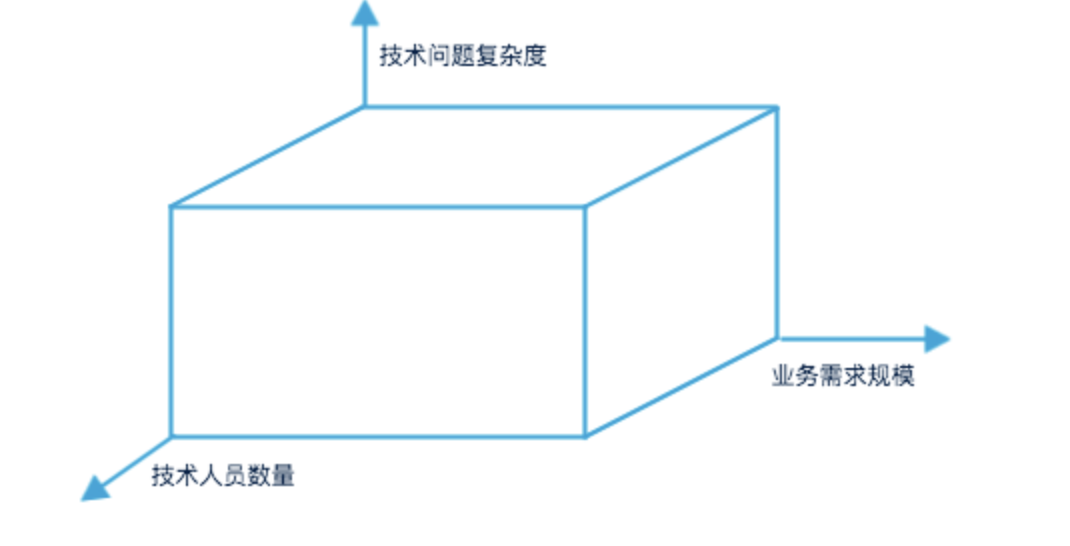
\includegraphics[width=.6\textwidth]{fig/DIDI_Pressure_1.png}
\end{figure}

2016年的滴滴,正在经历这样的阶段,一方面日单量从百万冲到千万,另一方面IT系统屡次出现线上故障,稳定性建设成为支撑业务发展的重要保障。在此背景下,滴滴启动了全链路压测项目。

\section{压测方案}
滴滴的业务与普通电商差别较大,一次典型的用户打车流程是这样的:乘客发单,0-3分钟内派给附近的司机,司机抢单后,去接乘客,到达目的地。这不但要求司乘的位置相近,而且交易必须是实时的。

基于滴滴业务的特殊性,同时借鉴了业内的经验,我们制定了滴滴的全链路压测方案,一句话描述就是:在线上环境,针对全业务核心链路,以数据隔离的方式进行压测,如下图表示:
\begin{figure}[H]
    \centering
    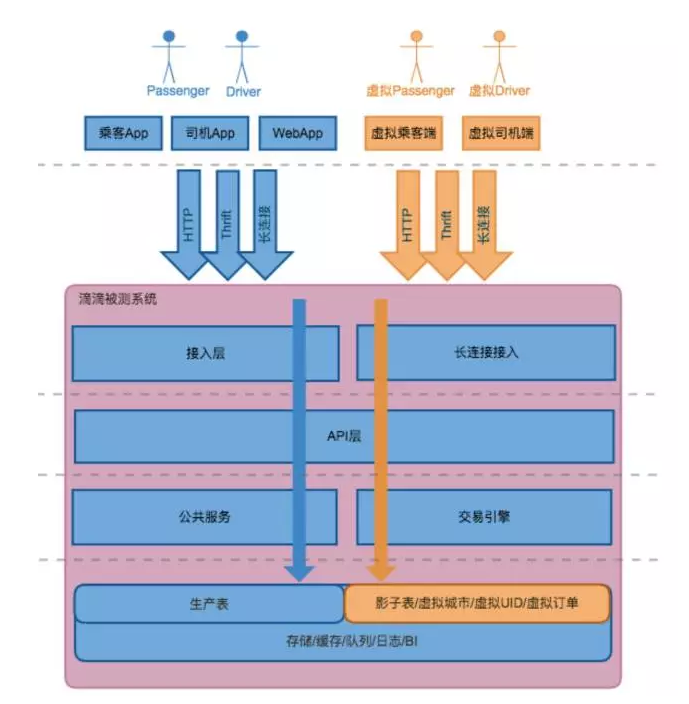
\includegraphics[width=.8\textwidth]{fig/DIDI_Pressure_2.png}
\end{figure}

\subsection{线上环境}
基于阿里等公司之前的经验,压测在线上环境进行,线上最大的优点就是环境真实,不需要担心配置不一致、结果是否可以同比例放大等问题,压测的结果自然也更为精确。但在线上做压测,需要保证安全性,风险不言而喻:不能搞垮线上系统。压测的时间窗口限定在低峰期;监控必须给力,在系统出现单点故障前,要能够提前预警,万一真的出现故障,必须紧急停止压力,最短时间内进行恢复。

\subsection{全业务核心链路}
支持出租车、专车快车、顺风车等几个主要的业务线,覆盖主要的业务场景,以出租车为例,从乘客打开App输入上车点、目的地、发单,到司机出车、抢单、接乘客上车、到达目的地,甚至取消订单等完整流程:
\begin{figure}[H]
    \centering
    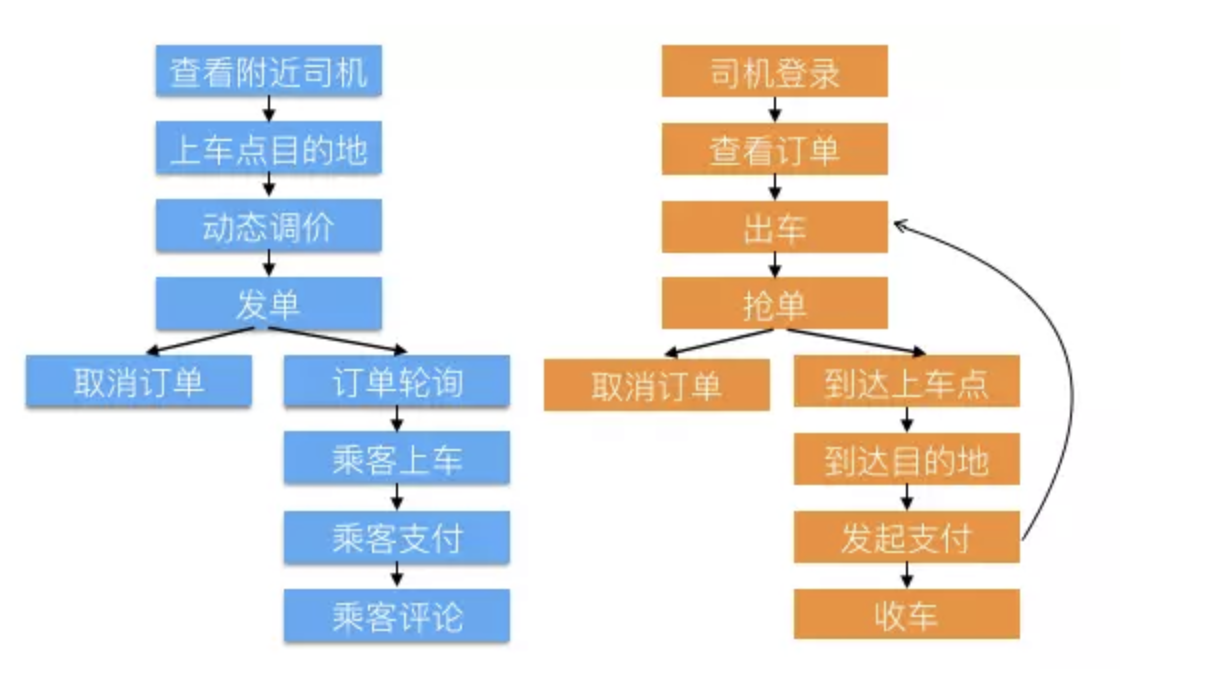
\includegraphics[width=.8\textwidth]{fig/DIDI_Pressure_3.png}
\end{figure}

\subsection{数据隔离}
压测方案的核心是数据隔离,压测司乘要与真实司乘区分,压测订单不能与真实订单混淆,绝不能把真实乘客的单派给虚拟司机等问题。下面将专门介绍压测的数据隔离方案。

\subsubsection{数据隔离方案}
与其谈隔离方案,不如让我们想象几种数据隔离不好的场景:
\begin{enumerate}
\setlength{\itemsep}{0pt}
\setlength{\parsep}{0pt}
\setlength{\parskip}{0pt}
    \item 某真实司机的历史订单突然多了一些假订单,积分、券、余额等出错;
    \item 某真实乘客的订单被派给了虚拟司机,乘客一直在等待司机来接;
    \item 某城市的BI报表出错,莫名其妙的多了一些订单,貌似财务也对不上;
    \item 某城市的运力估计及动调出现异常波动;
    \item 清理虚拟订单及相关数据时,不小心误删了真实订单和数据......
\end{enumerate}

虚拟订单方案:隔离不好的场景,光是想想就不寒而栗,可以让我们轻易排除这种看似最简单的方案:使用真实司机乘客,发送虚拟订单。虚拟订单通过ID或者标志字段进行区分,派单时做特殊处理。这种方式对业务有较大的侵入性,不仅是修改派单那么简单,还需要从各个维度适时地屏蔽司乘与虚拟订单的关系,如订单历史、通知推送、积分统计等,不但多而且是强依赖,显然不是一种合理的方案。

提升虚拟的层次: 每个城市启用一批虚拟的乘客,发送虚拟订单,派发给虚拟司机,司乘及订单上通过ID或者标志字段进行区分。这可以解决司乘及订单强依赖的问题。但从城市的角度看,需要隔离真实司乘与虚拟司乘,又会涉及到城市的动态调价、供需预测、BI统计等各个方面的隔离。

再提升虚拟的层次:与传统电商不同,Uber、滴滴这样的出行平台,都是按城市运营的,通过配置的方式开城,从而实现业务的横向快速扩展。那有没有可能在中国开辟一个甚至多个虚拟的城市呢,压测只在虚拟城市进行呢? 开辟虚拟城市,可以避免前面提到的诸多问题,尤其是隔离问题,但需要考虑虚拟乘客发布路线、虚拟司机地图导航的问题,城市的位置、道路怎么模拟?干脆再进一步,虚拟一个完整的中国了,看似比较疯狂,但这就是滴滴全链路压测时的隔离方案:

在某虚拟国家,有很多虚拟的城市,每个虚拟城市都有一群虚拟的司机和乘客,他们使用虚拟的手机号和客户端,进行线上交易,由此产生了虚拟的订单。

仍然要解决位置、道路的问题,我们把中国的坐标全部偏移到太平洋,“太平洋足够大,完全容得下中美两个国家”,那一个中国自然不再话下。虚拟城市的位置、道路,把真实城市偏移一定的经纬度就可以。

\subsubsection{压测流量标记方案}
考虑这样的场景:在新开辟的虚拟城市,某虚拟的乘客要打车,他打开虚拟的手机端,输入目的地,点击“立即预约”,请求发送到滴滴的后台系统,后台应该怎么样处理? 谈论方案之前,不如先了解一下现状:
\begin{figure}[H]
    \centering
    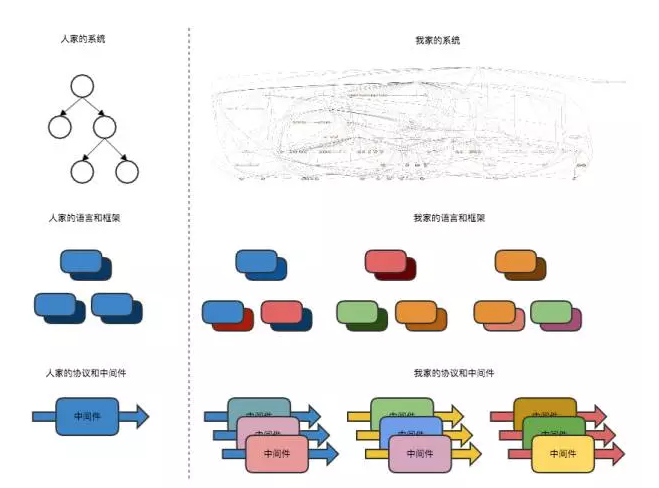
\includegraphics[width=1\textwidth]{fig/DIDI_Pressure_4.png}
\end{figure}

传说有一种系统叫别人家的系统,有一个语言叫别人家的语言,有一种协议叫别人家的协议,正所谓人比人气死人,回头看看自己家的,虽然与很多前辈不敢相提并论,但已号称四大语言八大框架,这个锅得让历史遗留问题来背,而这段历史,只有短短的几年而已。

也有好消息,与google的dapper、阿里的鹰眼类似,滴滴内部有一套自己的trace系统,专门用来跟踪系统之间调用链路,其基本原理如下图所示:
\begin{figure}[H]
    \centering
    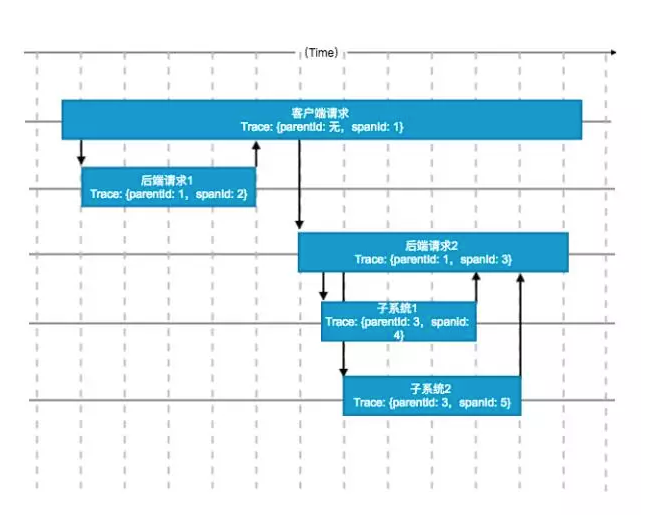
\includegraphics[width=1\textwidth]{fig/DIDI_Pressure_5.png}
\end{figure}

但并不全是好消息,全链路压测启动的时候,Trace系统在滴滴内部并未完全推广,不少系统不支持。压测流量标记方案面临两重选择:
\begin{enumerate}
\setlength{\itemsep}{0pt}
\setlength{\parsep}{0pt}
\setlength{\parskip}{0pt}
    \item 每个系统使用业务ID或标记来判断压测流量,只要能拿到司乘、订单等业务数据,系统就可以正确区分;
    \item 扩展Trace通路,在通路上添加压测标记,统一使用Trace来判断压测流量。
\end{enumerate}

最终我们选择了方案2,不但与业务完全解耦,还可以避免方案1中某些系统或接口无法拿到业务标记的情况。而且这种方式,客观上也可以推进Trace通路在公司的应用。

做不到语言和框架收敛,尽量让中间件收敛,为每种语言提供一个基础组件类库,中间件尽量收敛到该类库。
\begin{figure}[H]
    \centering
    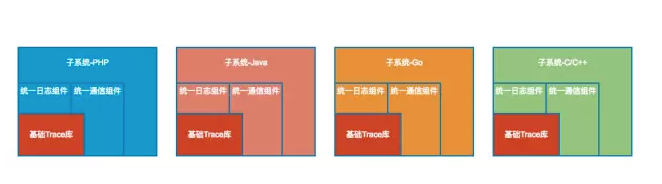
\includegraphics[width=1\textwidth]{fig/DIDI_Pressure_6.png}
\end{figure}
于是结合全链路压测,开始了内部系统痛苦的改造之路,最终基于Trace通路的压测标记在主要系统之间可以跑通。

\subsubsection{工具端方案}
链路已通,该考虑工具端的实现方案了,内部我们管工具端叫做虚拟的“司机端”和“乘客端”,可以用来模拟批量甚至大量的用户,而不仅仅是一个用户。

分布式的虚拟司乘端: 滴滴的客户端与后台通信,不仅仅有HTTP协议,还有TCP长连接,甚至还有Thrift协议。拿司机来说,接单等消息是通过TCP长连接下发的,意味着TCP长连接协议是必须的,而且需要为每个司机维护一个长连接。

考虑到需要模拟的司乘数量,虚拟的司机端、乘客端是分布式部署的,每个司乘端从数据中心获取司乘用户,包含基本信息、乘客路线、司机起始位置等信息,并且模拟批量司乘的发单等行为。使用数据中心的目的是,当端需要扩展时,拉取的司乘不能重复,不然重复登录可能导致被踢下线。

\begin{figure}[H]
    \centering
    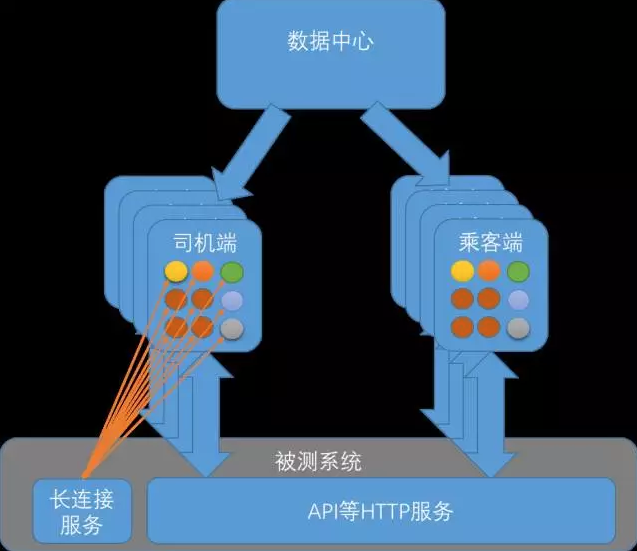
\includegraphics[width=.6\textwidth]{fig/DIDI_Pressure_7.png}
\end{figure}

可动态调整的业务模型: 虚拟端要模拟相对复杂、实时的交易模型,并且需要模拟不同的业务场景,以顺风车举例,平日高峰期的订单多为市内订单,而节假日的跨城订单比率增加很多。如何在不改代码的情况下可以压测不同的业务场景?我们实现了可动态调整的业务模型。
\begin{figure}[H]
    \centering
    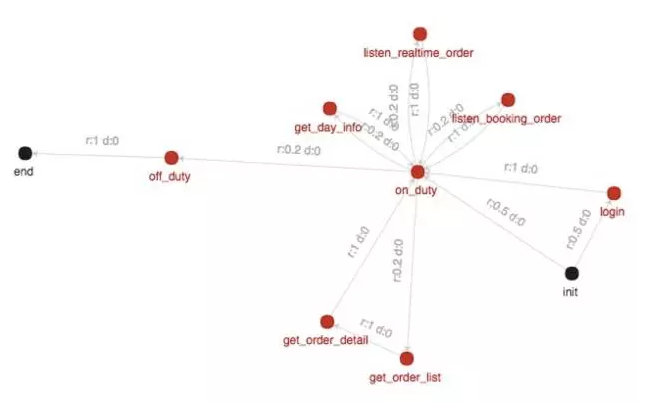
\includegraphics[width=1\textwidth]{fig/DIDI_Pressure_8.png}
\end{figure}

该模型中,司乘基本的交易过程、状态变化可以通过模型编辑完成,通过权重,可以调整用户本地单、跨城单的比例。即使更多的业务场景,只需生成业务模型即可支持。

更多实现细节: 当然除了上面提到的,方案上还有很多细节需要考虑。为了与线上实际场景更贴近,我们从线上高峰期截取了一段时间内的乘客路线和司机位置,分阶段压测时,逐渐投放更多的司乘到虚拟城市,但这样有一个问题。

假设A城市有1万司机,高峰期有1万乘客在发单,他们都是随机而均匀分布的,如果把全部司机瞬间投放完成,所有乘客立即发单,绝大多数订单应该是可以派出并完成交易的。

但是考虑分阶段投放的场景:投放1\%的司乘,上百名司机,上百个订单,虽然司机位置、乘客路线来自线上真实订单的采样,由于位置的随机性,成单量可能很少。即使投放了10\%,上千名司乘,实际成单量也远远达不到1000个。
\begin{figure}[H]
    \centering
    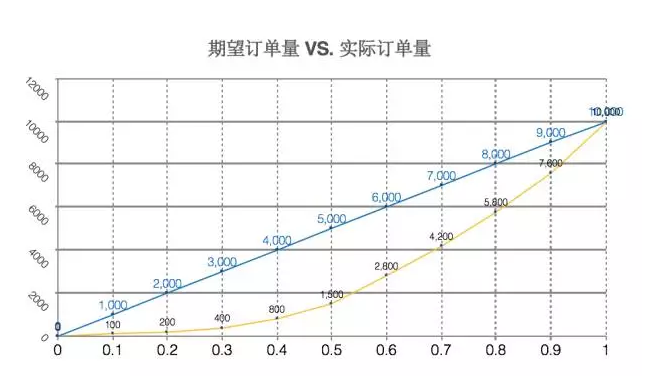
\includegraphics[width=.6\textwidth]{fig/DIDI_Pressure_9.png}
\end{figure}

而我们分阶段投放要求的10\%,不光是投放数量达到线上10\%,也期望成单量等数据同步达到10\%,这样才能验证工具端方案是否合理、线上压力是否正常。

在这里,我们采用了一个简单的算法:东单是北京的一个热点区域,第一个司机、乘客投放在东单,基本上可以保证成单;前1000名司机、乘客投放在东单附近,成单量虽不能上千,但比完全随机要好很多。控制好司乘投放的位置,基本可以保证成单量与投放数量成比例增长。

\section{压测实录}
2016年上半年是滴滴Uber合并前最后的疯狂,运营活动频繁,业务峰值不断攀升,平台出现的线上事故也较为多些。
\begin{figure}[H]
    \centering
    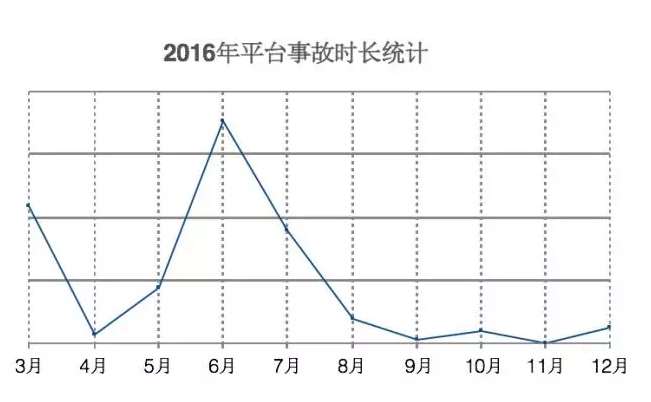
\includegraphics[width=.6\textwidth]{fig/DIDI_Pressure_10.png}
\end{figure}

从2016年中项目启动,经过多次尝试、探索,终于在线上成功进行了全链路压测。为了不影响线上业务,压测的窗口期选择在凌晨,并且严格掌控压测节奏,把压测过程划分成几个不同阶段,逐渐提升压力,边压测边监控后台系统的压力:
\begin{figure}[H]
    \centering
    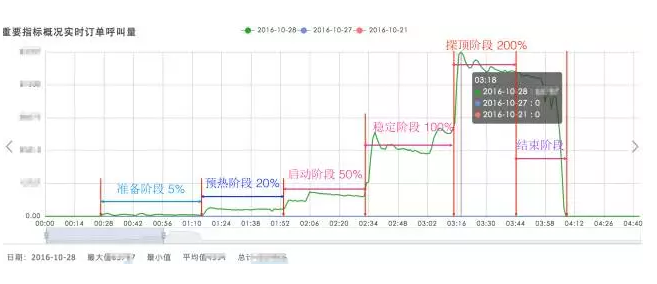
\includegraphics[width=1\textwidth]{fig/DIDI_Pressure_11.png}
\end{figure}

几个主要的业务线先后进行了十余次压测,并发现一些线上问题,如某API接口耗时明显增长;长连接服务器的参数配置有误;分单服务codis访问超时;日志过多导致分单算法超时等。

除了验证线上系统的稳定性,全链路压测项目还带来一些附加的收益:
\begin{itemize}
\setlength{\itemsep}{0pt}
\setlength{\parsep}{0pt}
\setlength{\parskip}{0pt}
    \item 不同语言下的基础组件类库趋向收敛,Trace通道覆盖了更多模块;
    \item 建立了一套完整隔离的线上环境,未来可以在线上做更多正确性验证。
\end{itemize}

现在的滴滴,越来越重视平台稳定性,对事故的预警、降级处理和事故处理预案越来越成熟,事故时长也明显缩短,但仍然存在单点故障、鲁棒性不高等潜在风险。展望将来,期望全链路压测能在更多领域发挥作用:线上环境的故障注入和故障演练;线上灰度发布环境的正确性验证;线上系统的容量预估等。

%\printbibliography
\bibliography{../ref}
\bibliographystyle{IEEEtran}
\end{document}